% !TEX root = ../report.tex

\chapter{Evaluation}
\label{evaluation}
\minitoc

\clearpage
	% What evaluation methodologies exist?
		% Offline Evaluation
		% 	Recommender System Datasets
		%		Explicit vs. Implicit
		% 	Offline Evaluation Measures
		%		Traditional evaluation measures
		%		Cold-start system evaluation
		%		Implicit feedback evaluation measures
		% Online Evaluation


%Some key questions in evaluating recommender systems on testbed data are: what
%to predict, how to grade performance and what baseline to compare with.

In many cases a system designer that wished to employ a recommender system must
choose between a set of candidate approaches. A first step towards selecting an
appropriate algorithm is to decide which properties are the most important for
the application. Recommender systems have a variety of properties such as
accuracy, robustness, scalability, etc. The following section will discuss how
to compare recommender systems based on the set of properties  relevant for the
application and how to evaluate the performance of the system. We have several
different experimental settings which can be used to evaluate recommender systems.
We will focus on two types of experiments:
Offline experiments where the system is evaluated without user interactions and
Online experiments where real users interact with the system. This section will
also cover some of the most frequently used evaluation metrics, a discussion on
the suitedness of different evaluation measures for implicit feedback, and
summary of the methodologies and evaluation measures used to evaluate the
cold-start performance of recommender systems.

Shani et al.\ \cite{Shani2011} lists the following guidelines for general
experimental studies:

\begin{itemize}
	\item Hypothesis: before running an experiment one must form an hypothesis. For
		example, an hypothesis can be that algorithm $A$ better predicts user ratings
		than algorithm $B$. In that case the experiment should test the prediction
		accuracy, and not look at other factors.

	\item Controlling variables: when comparing a few candidate algorithms on a
		certain hypothesis, it is important that all variables that are not tested
		are fixed.

	\item Generalization power: when drawing conclusions from experiments, we may
		wish that our conclusions generalize beyond the immediate context of the
		experiments. When choosing an algorithm for a real application, we may want
		our conclusion to hold on the deployed system, and generalize beyond the
		experimental data set. To increase the probability of generalization of the
		recommender results one must typically experiment with several data sets or
		applications.
\end{itemize}

\section{Offline Evaluation}
Offline experiments are performed using pre-collected dataset\(s\) and a protocol
that models the user behavior to estimate recommender performance through
different evaluation measures. Offline experiments are attractive because they
require no interactions with real users, and thus allows multiple  researchers to compare
a wide range of algorithms, using the same data, at a low cost. The downside of offline experiments
is that they can answer a very narrow set of questions, typically questions
about the predictive power of the algorithm, and does not measure other user
factors.

\subsection{Datasets for Offline Evaluation}
The main aim of a recommender system is to identify the set of items in a
dataset that might be interesting to a user based on their expressed
preferences. For a fashion recommender this would mean estimating how much a
user might like an item, by e.g.\\ predicting what rating a user might give an
item. In recent years, various test collections for different domains such as
books, music, movies have been made available to the public. These datasets
usually consist of user ratings in the form of $<UserID, ItemID, Rating>$.

In recent years more or more datasets have been made available which contains
additional information such as demographic information about the users,
trust-networks, user-assigned tags and etc. Under we have listed a few selected
popular datasets containing additional information:

%TODO - Find more cool dataset

\begin{itemize}

\item MovieLens 100k dataset~\cite{Movielens}: The movielens dataset
	incorporates demographic information about the user in addition the
	traditional rating matrix

\item Epinions dataset~\cite{Epinions}: The Epinions dataset includes a
	trust-network, which specifices who-trust-whom in a social network based on
	customer reviews for the website Epinions.com

\item The Million Song Dataset~\cite{Bertin-Mahieux2011}: The million song
	dataset is a implicit feedback dataset. This data also includes information on the users,
	and audio features and song meta-data.

\item The Book-Crossing Dataset: The bookcrossing dataset consists of both implicit and explicit feedback,
	demographic information about users and some content based information about the books.
\end{itemize}

\subsubsection{Explicit-feedback}
The definition of explicit is defined as `stated clearly and in detail, leaving
no room for confusion or doubt'. Explicit feedback are more precise than
implicit feedback, but more difficult to collect since it requires active user
involvement. One serious implication of this is that the amount of feedback
often is scarce since many users opt not to provide any feedback. Explicit
feedback mechanisms allow the users to unequivocally express their ratings on a
scale (usually in the form of a Likert scale (strongly disagree – strongly
agree). Thus explicit feedback is able to capture both negative and positive
feedback, while implicit feedback \emph{only} can be positive. It is worth
noting that explicit feedback tend to concentrate on either side of the rating
scale, as users are more likely to express their preference if they feel
strongly for or against an item~\cite{Jawaheer2010}.

\subsubsection{Implicit-feedback}
Unlike explicit feedback, we do not have any direct input from the user
regarding their personal preferences. In particular we do not have any
substantial evidence of which items the user dislikes, such as low ratings.
What we do have is indications of whether a user likes an item trough clicks, wants and purchases. Where wants and purchases can be viewed as a form of explicit rating only counting positively.
Implicit-feedback is more easily collected than explicit-feedback, and usually more abundant.
Types of implicit feedback include purchase history, browsing history,
search patters, or even mouse movements. For example, a user who purchases
many clothes from the same brand probably likes that brand. For a larger
discussion surrounding the differences between implicit and explicit
feedback, see Section~\ref{implicit-feedback}

\subsection{Validation Methods}
Validation techniques are motivated by two fundamental problems; model
selection and performance estimation. Almost all pattern recognition techniques
have one or more free parameters, and we want a way to select the
\emph{optimal} parameter\(s\) or model for a given problem. Once we have chosen a
model, we wish to estimate how well it is doing.

\subsubsection{The Holdout Method}
When using the holdout method you split the dataset into two groups; a training
set used to train the classifier and a test set used to estimate the error rate
of the trained classifier. The Netflix Prize Competition~\cite{Netflix}
provided a training set consisting of 100,480,507 ratings given by 480,189
users to 17,300 movies. The testset consisted of 2,817,131 items where the
ratings were unknown. The submitted predictions were scored against the true
ratings in terms of root mean squared error (RMSE), and the goal was to
minimize this error.

The holdout method has two basic drawbacks; (1) In problems with sparse
datasets we may not be able to afford the luxury of setting aside a portion of
the dataset for testing, (2) Since it is a single train-and-test experiment,
the holdout estimate can be misleading if we happen to get an `unfortunate'
split.

\subsubsection{Cross-Validation}
K-fold Cross-Validation creates a K-fold partition of the dataset. For each of
the $K$ experiments, use $K-1$ folds for training and the remaining one for
testing. By setting $K=2$, this is the same as the holdout method. The estimated
error is found by taking the average error from all the experiments.

Leave-one-out is the degenerate case of K-fold Cross-Validation, where $K$ is
chosen as the total number of examples. For a dataset with $N$ examples we
perform $N$ experiments. For each experiment we use $N-1$ examples for training
and the remaining example for testing. Again, the true error is found by taking
the average error rate from the experiments.

In practice the number of folds often depends on the size of the dataset. For
large datasets, even 3-Fold Cross Validation will be quite accurate, which for
sparse datasets, one may wish to train as many examples as possible. A common
choice is $K$ value between 5 and 10.

\paragraph{Advantages}
One positive aspect with k-fold cross-validation is that the result is averaged over the $K$ experiments. The strongest argument for using cross-validation is the potential of using the entire training set for testing (albeit not at once), creating the largest possible test set for a fixed training data set.

\paragraph{Disadvantages}
The main disadvantage with K-fold Cross-Validation is the training algorithm has
to be run $K$ times, and thereby increasing the runtime for producing an
evaluation of the system. If the dataset is large, an increase of $K$ runs could
prove to be disadvantageous.
%TODO - more?

\subsubsection{Bootstrapping~\cite{efron1994introduction}}
Bootstrapping is used to estimate properties of an estimate, such as bias, variance, confidence, intervals and prediction error.
This is done trough measuring these properties when sampling from an approximated distribution.
For instance an empirical distribution of the observed data.
The idea is that with information from sample data it is possible to say something about the population.
The sample data is a subset of the population.
Since the population is unknown it will not be possible to calculate the true error from the sample data.
To handle this the
Since it will not be possible to perform inference on:
\emph{sample data} $\rightarrow$ \emph{population} this is modeled as:
\emph{re-sample data} $\rightarrow$ \emph{sample data}.
The \emph{re-sample data} is a re-sampling of the sample data.

In practice an example to bootstrapping is when we want to calculate the average height of the population worldwide.
The issue here is that it is not as doable to measure everyone, so a subset of the population is used.
Since the average on this number only will be an estimate of the actual world wide average a sense of error margin must be introduced.
Bootstrapping is then used to reduce the error of margin through re-sampling the sample data a large number of times~\footnote{Numbers vary on sample size, but is often 1 000 to 10 000}, and new averages are calculated.
With these averages a histogram can be produced, which provides an estimate of the distribution of this average.

\begin{figure}[H]
    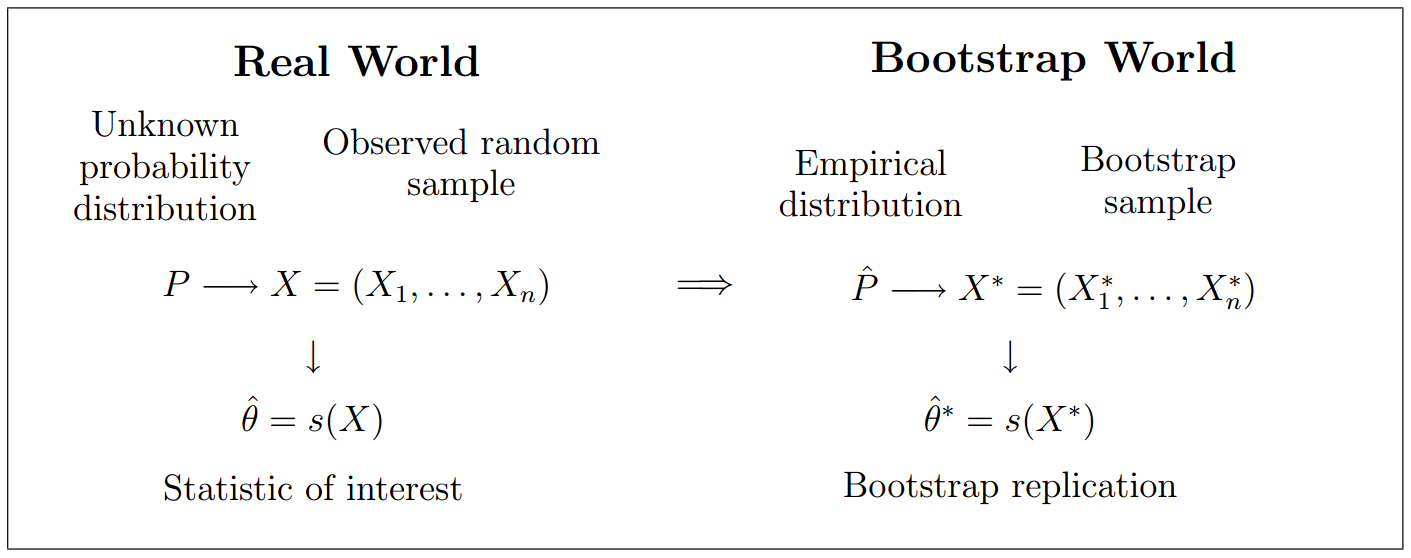
\includegraphics[width=5in]{image/bootstrap.png}
    \centering
    \caption[Bootstrapping principles]{A figure of the principles bootstrapping. Taken from~\cite{Eichler2003}}
    \label{figure:bootstrapping}
\end{figure}

\paragraph{Disadvantages}
	One prominent issue with bootstrapping is that important properties of the actual data might not be caught when undertaking the bootstrapping analysis
	~\footnote{"Bootstrapping" comes from the phrase, "to pull oneself up by one's bootstraps"~\cite{bootstrapSaying1843}}.


\subsubsection{Finding the optimal parameter settings}

Finding the optimal parameters for a model is usually a crucial task in engineering approaches to classification and modeling tasks. An automated approach is particularly desirable when the number of parameters are high. In order to work well many algorithms and modeling techniques in computer science rely on a careful choice of their parameters. The usual approach is to select parameters based on some prior experience on the problem at hand with a limited heuristic search of possibly optimal parameters. When such prior knowledge is absent or cannot be directly applied to the technique being used, the optimal parameters have to be found either by \emph{blind} search, by e.g. using genetic algorithms or some kind of grid-search procedure.

The \emph{de facto} standard way of performing model selection optimization is grid search, which is simply an exhaustive searching through a manually specified subset of the hyperparameter space of a learning algorithm. To \emph{guide} the grid-search one typically uses a performance metric, typically measured by cross-validation on the training set. After evaluating the performance all the pre-specified combinations of parameter settings, the grid search algorithm outputs the setting that achieved the highest score in the validation procedure.

Many of the most popular Machine Learning libraries now come with methods for performing grid search.

\subsection{Offline Evaluation Metrics}
When evaluating a recommender system, you wish to estimate a user's
satisfaction for a given recommendation. Traditionally recommender systems have
been evaluated by means of predictive accuracy. However, there is now a widely
agreed that accurate predictions are crucial but insufficient to deploy a good
recommendation engine~\cite{Shani2011, McNee2006}. Some of the properties can
be traded-off, one such example is the trade-off between accuracy and
diversity. It is important to understand and evaluate these trade-offs and
their effect on the overall performance. This subsection will cover the most
popular metrics used for offline evaluation, a discussion of evaluation
measures for implicit feedback, and a summary of the cold-start evaluation
methodologies found in the literature.

\subsubsection{Predictive Accuracy Metrics}
Predictive accuracy metrics measure how close the predicted ratings are to the
true user ratings. More formally, the system tries to predict ratings
$\hat{r(c,i)}$ for a test set $T$ of user.item pairs $(c, i)$ for which the
true ratings are known. Traditionally, mean absolute error (MAE) has be used to
evaluate the performance of collaborative-filtering algorithms, but other
measures such as root mean squared error (RMSE) are also commonly used.

\paragraph{Mean Absolute Error (MAE)}
MAE measures how close the predictions are to the actual outcome.
\begin{equation}
    MAE = \frac{1}{n}\sum_{i=1}^{n}{|\hat{r(c,i)}-r(c,i)|}
    \label{equation:mae}
\end{equation}
$r(c,i)$ is the actual outcome and $\hat{r(c,i)}$ is the predicted value.
As the name suggest, $MAE$ calculates the average absolute error.

\paragraph{Root Mean Squared Error (RMSE)}
Often used to measure difference between a set of predicted values with a set of actual values.
\begin{equation}
    MSE = \frac{1}{n}\sum_{i=1}^{n}{(\hat{r(c,i)} - r(c,i))^{2}}
    \label{equation:mse}
\end{equation}
\begin{equation}
    RMSE = \sqrt{MSE}
    \label{equation:rmse}
\end{equation}
In $MSE$~\ref{equation:mse} $\hat{r(c,i)}$ is the predicted value and $r(c,i)$ is the actual value.
Both $MAE$ and $MSE$ are used to measure how correct the predictions are compared to the actual values.
$RMSE$ is the square root of $MSE$ and is one of the most used metrics to compare recommender algorithms in collaborative filtering, and was the main metric used in the Netflix price competition to evaluate the performance of the competitors recommender systems.
$RMSE$ is always bigger or equal to $MAE$, $RMSE$ penalize an error more than $MAE$.

% \todo{maybe some sweet table of the different algorithms with their eqations and their contributions}
% \begin{table}[H]
%     \centering
%     \begin{tabular}{l|l|l}
%     	% \rowstyle{\bfseries}
%     	Metric	& Equation & About \\ \toprule
%     	MEA 			& \parbox{6cm}{\equationMEA} & safd \\	\hline
%     	RMSE 			& \parbox{6cm}{\equationRMSE} & asdf \\
%     \end{tabular}
%     \label{table:predictiveAccuracyMetrics}
%     \caption [Predictive Accuracy Metrics]{adsf}
% \end{table}



\subsubsection{Measuring Usage Prediction}
\label{para:measuring_usage}
% \subsubsection{Decision Based Metrics}
In many applications the recommender system does not predict the user's
preferences of items, but tries to recommend to users items that they may use.
This is often done by giving the user a top-K set of recommendations.
In an offline evaluation of usage prediction, we typically have a dataset
consisting of items each user has used. We then select a test user, hide some
of her selections, and ask the recommender to predict a set of items the user
will use. We then have four possible outcomes for the recommend and hidden
items.

\begin{table}[H]
	\centering
	\begin{tabular}{l|l|l}
					&	Relevant			&	Not Relevant \\ \hline
	Recommended		&	True-Positive (TP) 	&	False-Positive (FP)	\\ \hline
	Not Recommended	&	False-Negative (FN)	&	True-Negative (TN)	\\ \hline
	\end{tabular}
	\label{table:usageprediction}
	\caption[Usage prediction (Confusion Matrix)]{This table is showing the different categories recommended items can end up in.}
\end{table}

\begin{table}[H]
	\centering
	\begin{tabular}{l|l}
		True-Positive (TP)	& The recommended item is of interest to the user \\ \hline
		False-Positive (FP)	& The recommended item is not of interest to the user \\ \hline
		False-Negative (FN)	& The item is of interest to the user, but is not recommended \\ \hline
		True-Negative (TN)	& The item is not of interest to the user, but is not recommended \\
	\end{tabular}
	\label{table:predictionCategories}
	\caption[Prediction Categories]{}
\end{table}

This model assumes that not relevant items would not have been relevant if they had been
recommended to a user. This assumption may be false, such as when the set of
not relevant items contains some interesting items that the user did not select. For
example, a user may not have relevant an items because she was unaware of its
existence, but after the recommendation exposed that item, the user can decide
to select it. We can count the number of examples that fall into each cell in
the table and compute the Precision, Recall, Fallout and $ROC$.

\paragraph{Precision}
Precision is the amount of the actually true positives recommended, over the amount of all the items recommended.
\begin{equation}
    Precision = \frac{TP}{TP+FP}
    \label{equation:precision}
\end{equation}

\paragraph{Recall}
Recall is the ratio of the items of interest for the user which actually where recommended to the user.
\begin{equation}
    Recall = \frac{TP}{TP+FN}
    \label{equation:recall}
\end{equation}

\paragraph{Fallout}
Fallout is the amount of retrieved items which is not relevant amongst all the non relevant items (false positive).
\begin{equation}
    Fallout = \frac{FP}{FP+TN}
    \label{equation:fallout}
\end{equation}

\paragraph{F-measure}
F-measure combines the precision and the recall.
\begin{equation}
    F_\beta = \frac{(1 + \beta^2) * (Precision * Recall)}{(\beta^2 * Precision + Recall)}
    \label{equation:f-measure}
\end{equation}
Based on the value of $\beta$ F-measure will weight precision or recall more. For a $\beta$ over 1 F-measure will emphasize precision over recall, and opposite for $\beta$ between 0 and 1.

\paragraph{Accuracy}
Accuracy is the amount of correctly recommended items over all the items.
\begin{equation}
    Accuracy = \frac{TP+TN}{TP+TN+FP+FN}
    \label{equation:accuracy}
\end{equation}

\paragraph{Receiver Operating Characteristics (ROC))}
The $ROC$ is the recall rate ($TPR$) against the fallout rate ($FPR$).
The goal is to maximize the recall while minimizing the fallout.
\begin{equation}
    TPR(T) = \int_T^\infty P_0(T)dT
    \label{equation:tpr}
\end{equation}
\begin{equation}
    FPR(T) = \int_T^\infty P_1(T)dT
    \label{equation:fpr}
\end{equation}
$T$ is a threshold parameter.
The ROC curve is $TPR$ plotted together with $FPR$ at various $T$.
\begin{equation}
    AUROC = \int_\infty^{-\infty} TPR(T)P_0(T)dTdT
    \label{equation:auroc}
\end{equation}
Equation~\ref{equation:auroc} can be used to calculate the area under the curve.
$AUROC$ is the probability that the recommender system will rank positive examples higher than negative examples.

\paragraph{Limitations}
\label{subp:limitations}
As mentioned by Powers et al.~\cite{powers2007}, recall, precision, F-measure and rand accuracy have a bias.
Another drawback or limitation with the measuring of user predictions is that it does not take into account the ranking of the items.
To handle this, rank based metrics can be used.

\subsubsection{Accuracy Ranking} % (fold)
\label{par:accuracy_ranking}
\marginpar{if this is the setup, write a little intro}
\paragraph{Mean Percentage Ranking (MPR)}
\label{subp:mean_percentage_ranking_}
This measure is a recall-oriented metric.
A known issue with implicit feedback is that it often lack the actual user's preference.
This approach is used to measure the user satisfaction of items in an recommended ordered list.
\begin{equation}
	MPR = \frac{\sum_{u,i}{r_{ui} * rank_{ui}}}{\sum_{u,i}{r_{ui}}}
	\label{equation:mpr}
\end{equation}
How to calculate $MPR$ is shown in~\ref{equation:mpr}.
A list of all the items for user $u$ is ordered based on the rank $rank_{ui}$ of the $u$.
Where $rank_{ui}$ is the percentile rank of item $i$ in this list for $u$.
$rank_{ui} = 0$ means that $i$ is the most preferred item for $u$.
$r_{ui}$ indicates whether $u$ has consumed $i$ or not.
This makes a $MPR$ value of 0\% to be the most preferred value, and a value of 50\% meaning a near randomly produced list.

\paragraph{Mean Average Precision (MAP)}
\label{subp:mean_average_precision_map_}
MAP~\cite{Manning:2008:IIR:1394399} measures quality across recall levels.
\begin{equation}
	ap@n = \sum_{k=1}^{n}{\frac{P(K)}{min(m,n)}}
	\label{equation:apn}
\end{equation}
\begin{equation}
	MAP@n = \sum_{i=1}^{N}{\frac{ap@n_i}{N}}
	\label{equation:map}
\end{equation}
How to calculate the $MAP$ value is shown in~\ref{equation:map}.
\ref{equation:apn} calculates the average precision at $n$ for a user.
From \ref{equation:apn}, $P(K)$ is the precision at $k$ in the item list, $n$ is the maximum number of predicted items and $m$ is the actual length of the predicted items list.
\ref{equation:map} calculates the mean of all the values from \ref{equation:apn}.

\paragraph{Normalized Discounted Cumulative Gain (nDCG)}
\label{subp:normalized_discounted_cumulative_gain_}
$nDCG$ measures the graded relevance of the recommended item, the ranking quality or the usefulness of the recommended item based on its rank position.
It is often used to measure the performance of web search recommendation systems.
\begin{equation}
    DCG_k = \sum_{i=1}^{k}{\frac{2^{rel_i}-1}{log_2(i+1)}}
    \label{equation:dcg}
\end{equation}

\begin{equation}
    nDCG_k = \frac{DCG_k}{IDCG_k}
    \label{equation:ndcg}
\end{equation}
How to calculate the $nDCG$ value is shown in~\ref{equation:ndcg}.
Where $k$ is the maximum amount of suggested items, and $rel_i$ is the graded relevance of the result at position $i$.
$IDCG_k$, from~\ref{equation:ndcg}, is the ideal $DCG_k$ value.
This is the result list sorted on relevance.

\paragraph{Half-life utility~\cite{Breese:1998:EAP:2074094.2074100}}
Assume that the further down an item is in the list the less chance there is for that item to be viewed by the user.
The rate of the decaying probability is exponential.
\begin{equation}
	HL_u = \sum_{i}{\frac{\delta(i)}{2^{\frac{i-1}{\alpha-1}}}}
\end{equation}
$\delta(i)$ is 1 if the user is interested in the item at position $i$ and 0 if not.
$\alpha$ is the viewing half-life, or half-life parameter.
The half-life utility of all the users are shown in~\ref{equation:HL}
\begin{equation}
	HL = 100 * \frac{\sum_u{HL_u}}{\sum_u{HL_u^{max}}}
	\label{equation:HL}
\end{equation}
$HL_u^{max}$ is the maximum possible value of the half-life utility value.
% \paragraph{Limitations}
% todo maybe
\marginpar{some overlapping of the algorithms (not really comparing two ranked list, but still evaluating a recommender system producing ranked lists)}

\marginpar{something like this perhaps}
% paragraph accuracy_ranking (end)

\subsubsection{Rank Based Metrics}
\label{para:rank_based}
Rank accuracy metrics measure the ability of a recommendation method to produce
a recommended ordering of items that matches how the user would have ordered
the same items. Shani et al.~\cite{Shani2011} lists two different approaches
for measuring the ranking accuracy: Try determining the correct order of a set
of items for each user and measure how close a system comes to this correct
order, or we can attempt to measure the utility of the system's ranking to a
user.

Herlocker et al.~\cite{Herlocker2004} argue that rank accuracy metrics may be
overly sensitive for domains where the user just wants an item that is `good
enough' (binary preferences) since the user won't be concerned about the
ordering of items beyond the binary classification. These metrics are therefore
most suitable to evaluate algorithms that are used to present ranked lists to
the user in domains where the user preferences are expressed using numerical
values.

\paragraph{AP correlation}
\label{subp:ap_correlation}
$AP correlation$~\cite{Yilmaz:2008:NRC:1390334.1390435} measures the overall precision and is a variant of $Kendall's$ $tau$.
It counts the amount of items correctly placed in a ordered predicted rank list $list1$ and a list of the actual rank ordering of the preferences of the user $list2$.
\begin{equation}
	AP = \frac{2}{N - 1} * \sum_{i=2}^{N}{(\frac{C(i)}{i - 1})} - 1
	\label{equation:ap}
\end{equation}
How to calculate the $AP correlation$ value is shown in ~\ref{equation:ap}.
$C(i)$ is the number of items ranked correctly above rank $i$.
The value of AP is between -1 and 1, where a score of 0 means that $list1$ can be considered a randomly generated list and 1 is a perfect match with the actual list $list2$.
% \paragraph{Limitations}
% todo maybe

\subsubsection{Beyond Accuracy}
There is an emerging understanding that good recommendations accuracy alone does not give the users of the recommender system an effective and satisfying experience \cite{Herlocker2004}. The following \emph{measures} attempts to assess a recommender systems usefulness beyond being able to provide accurate recommendations to the users.

\subsubsection{Coverage}
The term coverage can refer to several distinct properties of the system. Most
commonly, the term coverage refers to the proportion of items the
recommendation system can recommend, also known as \emph{item-space coverage}.
The simplest measure of catalog coverage is the percentage of all items that
can ever be recommended. Coverage can also be the proportion of users
interactions for which the system can recommend items, known as
\emph{user-space coverage}. In many applications the recommender system may not
provide recommendations for some users due to e.g.\\ low confidence in the
accuracy of predictions for that user. In such cases one may prefer a
recommender that can provide recommendations to a wider range of users. However, an increase in coverage is only beneficial if the accuracy does not drop significantly.

\paragraph{Perceived quality}
To gather the perceived quality the system must ask the user to examine the recommended item, and give feedback regarding the their actual interest in the recommended item.
For the feedback from the user to be as complete as possible, the system must supply the user with the reason to why the item was suggested, and the metadata of the item.
When the user has this overview of the item, the user's feedback regarding the item can produce some quality measure.
One  way of having the user to give this feedback is to re-rate the recommended item on a similar scale as the item was rated.
A rating scale from 1 to 5 is often used for both~\cite{Schafer:1999:RSE:336992.337035}.

\paragraph{Novelty and Serendipity}
Some recommender systems produce highly accurate recommendations and also have reasonable coverage - and yet that are useless for practical purposes. For instance, a music recommender can recommend Rihanna to every customer who have not yet listened to Rihanna. However, statistically, this is highly accurate as most people have listened to Rihanna or at least knows about her and have consciously chosen not to listen to her. Much more valuable would be a recommendation to a kick-ass indie-rock band that the active user would love, but will never hear about in the news. We therefore need a new dimension for analyzing recommender systems that consider "nonobviousness" of the recommendations. One such dimension is \emph{novelty}. Another related dimension is \emph{serendipity}. A serendipitous recommendation helps a user find a surprisingly interesting item the user might not have discovered otherwise. To clarify the difference between the two, a novel recommendation could be to recommend an unknown album from one of the users favorite artists, that the user likely eventually would have discovered herself. However, a recommendation by an unknown artist is more likely to be serendipitous. Serendipity is therefore a measure of how surprisingly the successful recommendations are.

As novelty is the the degree of new and interesting items recommended for the user, the system must ask the user for feedback to be able to make any assumptions around the novelty.
The novelty together with perceived quality allows the system to make informed decisions about the ratio of new items to recommend for the user.
The novelty is expected to change over time, some times the user would like to receive recommendation on new items, and other times recommendations closer to the user's preferences.
For the system to be able to detect these changes in preferences, and acting accordingly would be beneficial in regards of the user's satisfaction.
\begin{equation}
    Novelty(u) = \frac{1}{N}\sum_{i=1}^{N}{1 - Knows(u,i)}
    \label{equation:novelty}
\end{equation}
In~\ref{equation:novelty} $Knows(u,i)$ represents a binary functions which returns 1 if the user $u$ knows the item $i$, and 0 if not.
The set of items used for the calculation is the set of recommended items for the user.

The system should be able to produce items both items known to the user, and items unknown to the user.
For trust in the system and novelty respectively.

\begin{figure}[H]
    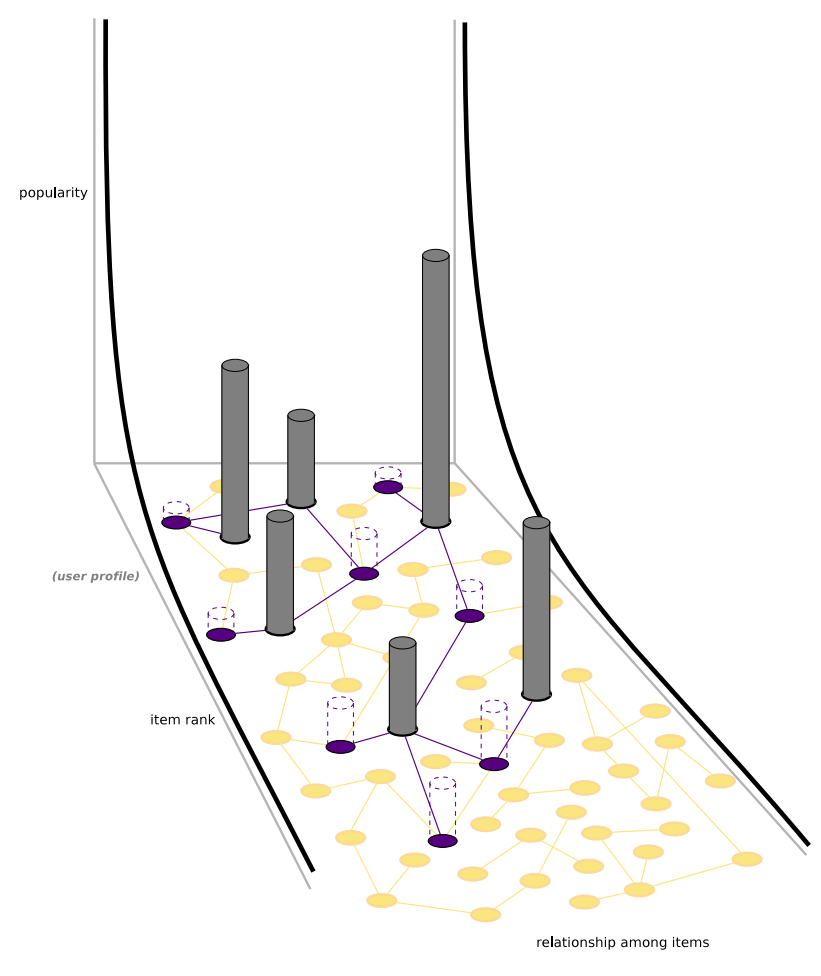
\includegraphics[width=5in]{image/longtailNoveltyFig.png}
    \centering
    \caption[Long tail]{Long tail show with the item similarity between items. Similarity shown though edges between the nodes. The gray columns represents the user profile, the violet represents items which might be of interest to the user, and the height is the relevance. Figure from~\cite{celma2008}}
    \label{figure:longtailNovelty}
\end{figure}
\marginpar{todo - not sure if its ok to use this image (not self made) figure from music recommendation, but long tail applies to fashion}
\marginpar{todo - if so, something about longtail}

\paragraph{Diversity}
Diversity is generally defined as the opposite of similarity. In some cases suggesting a set of similar items may not be as useful for the user, because it may take longer to explore the range of products. E.g. when presenting a list of 5 recommendations, the system should not recommend 5 Ralph Lauren shirts with different colors. As diversity may come at the expanse of other properties such as accuracy, one should evaluate the decrease in accuracy vs. the increase in diversity.

Other evaluation methods worth knowing about includes confidence, trust, utility, robustness, adaptivity, scalability mentioned in \cite{Herlocker2004, Shani2011}.

\subsection{Evaluation using Implicit Feedback}
Accuracy metrics such as RMSE and MAE are not especially well suited for implicit feedback datasets, as they require knowing which items are undesired by a user~\cite{Hu2008}.
One way to handle the issue with missing negative feedback is through conversion of the implicit feedback to explicit feedback, and thereby producing a sense of negative feedback.
One issue with this is what is considered as negative feedback in the sense of implicit feedback.
The reason for a user not to access an item is not necessarily grounded in dislike, but could simply be an overlook.
On the other hand, if the user accessed the item for a short time without buying it, the user might not like it.
These questions raises the need for a different approach when wanting to measure a recommender system using implicit feedback.

Joachims et al.~\cite{Joachims07evaluatingthe} shows that clicks can be biased, and has to be interpreted relative to the order of presentation and relative to the other abstracts.

\marginpar{extend}

Two ways of measuring the system is through ranking and usage prediction described earlier.


  \begin{center}
    \begin{tikzpicture}
		[node distance = 1cm, auto,font=\footnotesize,
		% STYLES
		every node/.style={node distance=1.5cm},
		% The comment style is used to describe the characteristics of each process
		comment/.style={rectangle, inner sep= 5pt, text width=3cm, node distance=0.25cm, font=\scriptsize\sffamily},
		% small comment lol
		comment-small/.style={rectangle, inner sep= 5pt, text width=1cm, node distance=0.25cm, font=\scriptsize\sffamily},
		% The nonProcess style
		nonProcess/.style={rectangle, draw, inner sep=5pt, text width=3cm, text badly centered, minimum height=1.2cm, font=\footnotesize\sffamily},
		% The process style is used to draw the processs' name
		process/.style={rectangle, draw, fill=black!10, inner sep=5pt, text width=3cm, text badly centered, minimum height=1.2cm, font=\bfseries\footnotesize\sffamily},
		% ratingsGenerator style
		ratingsGenerators/.style={rectangle, draw, fill=blue!50, inner sep=5pt, text width=3cm, text badly centered, minimum height=1.2cm, font=\bfseries\footnotesize\sffamily},
		% racommendation algorithms
		recAlgs/.style={rectangle, draw, fill=red!40, inner sep=5pt, text width=3cm, text badly centered, minimum height=1.2cm, font=\bfseries\footnotesize\sffamily}]

		% Draw processs
		\node [ratingsGenerators] (rg1) {sigmoid\_fixed};
		\node [ratingsGenerators, right=0.25 of rg1] (rg2) {sigmoid\_constant};
		\node [comment-small, right=0.01 of rg2] (dotdotdot) {..............};
		\node [ratingsGenerators, right=0.01 of dotdotdot] (rg3) {norm\_dist};

		\node [process, below of=rg2] (gt) {"Ground Truth"};

		\node [recAlgs, below of=gt] (ra2) {ALS};
		\node [recAlgs, left=0.25 of ra2] (ra1) {KNN};
		\node [comment-small, right=0.01 of ra2] (dotdotdot2) {..............};
		\node [recAlgs, right=0.01 of dotdotdot2] (ra3) {wALS};

		\node [process, below of=ra2] (eval) {Evaluation Score};

		% \node [nonProcess, below of=implicitConverter] (ratings) {Ratings for the items};
		% \node [process, below of=ratings] (recommendations) {Make recommendations};
		% \node [process, below of=recommendations] (evaluations) {Evaluate recommendations};
		% \node [nonProcess, below of=evaluations] (evaluationValue) {Recommendation score};

		%%%%%%%%%%%%%%%
		% Comments
		\node [comment, right=0.25 of rg3] (comment-rg3) {
			Implicit ratings
		};
		\node [comment, right=0.25 of ra3] (comment-ra3) {
			Recommendations algorithm
		};
		% \node [comment, right=0.25 of ratings] (comment-ratings) {
		% The output of the conversion is a set of ratings on the different items from the soBazar dataset
		% };
		% \node [comment, right=0.25 of recommendations] (comment-recommendations) {
		% Makes recommendations based on the inputed ratings. Different approaches to make the recommendations can be take, such as matrix factorization or neighborhood based approaches
		% };
		% \node [comment, right=0.25 of evaluations] (comment-evaluations) {
		% Evaluate the recommender system(s). Different evaluation metrics will be usea, such as e.g. AUC and nDCG
		% };

		%%%%%%%%%%%%%%%%
		% Draw the links between processs
		\path[->,thick]
			(rg1) edge (gt)
			(rg2) edge (gt)
			(dotdotdot) edge (gt)
			(rg3) edge (gt)
			(gt) edge (ra1)
			(gt) edge (ra2)
			(gt) edge (dotdotdot2)
			(gt) edge (ra3)
			(ra1) edge (eval)
			(ra2) edge (eval)
			(dotdotdot2) edge (eval)
			(ra3) edge (eval);
		% \path[>=latex,->] (gt) edge (eval);
		% \draw[rectangle connector=-3cm] (gt) to (eval);
		\draw[>=latex,->] (gt) -- +(-6,0) |- (eval);
    \end{tikzpicture}
    \captionof{figure}[Implicit Rating Evaluation]{Overview of how the generated ratings from the implicit feedback can be evaluated.}
  	\label{figure:implicitRatingEvaluation}
  \end{center}

	The blue boxes in figure~\ref{figure:implicitRatingEvaluation} are functions used to produce the implicit ratings based on the implicit feedback.
	Based on this, the system gets an estimated ground truth, which can be used to evaluate the different recommendation algorithms show in the red boxes.
	Based on the evaluation score something can be said about the implicit feedback conversion to implicit ratings and the recommendation algorithms used.

\subsubsection{Rank Based} % (fold)
	\label{par:Ranking_based}
	The ranking approach can be considered more suited to test recommendation systems using implicit feedback since a subset of the items are meant to be recommended to the user.
	This subset is usually a ranked top K list of items where the items in this list is the items the system predicts will be most liked by the user.

	One issue with this approach is that the items in the predicted top K list has to be ranked in some way, the same goes for the list this list is to be compared to.
	Thereby producing the requirement for a ranked list of preferred items from the user.
	If there is such a ranked list, ranking accuracy will help to tell how well the system is suggesting items for the user, such as~\cite{Yilmaz:2008:NRC:1390334.1390435}.
% paragraph paragraph_name (end)

\marginpar{maybe hard to differentiate between the names}

\subsubsection{Accuracy Ranking} % (fold)
	\label{par:usage_prediction}
	When there is lack of explicit user feedback and a ranked list of the items cannot be produced, ranking the predicted list and scoring this list based on the actual user preferences can be used to evaluate the system.
	The actual user preferences are based on a list of binary values regarding the items, interesting or not interesting.
	This list is often possible to construct from implicit feedback, but will seldom be a complete list, and most often be a list with only positives (not possible to produce not interesting).
	Some of the different approaches when dealing with implicit feedback are:
	Li et al.~\cite{deLace2010} who used $MPR$ and $MAP$ to calculate their performance.
	Pan et al.~\cite{Pan:2013:GGP:2540128.2540516} who used a set of top-k evaluation metrics: precision, recall, F1, nDCG, ROC and 1-call.
	Sindhwani et al.~\cite{Sindhwani:2010:OMC:1933307.1934641} who used roc curve and precision-recall curve to evaluate their experiments.
	Pan et al.~\cite{pan2008} who used $MAP$ and Half-life Utility.

	$nDCG$, $MAP$ and Half-life utility has a similar setup.
	They all have a decaying factor, and rewards the system in different ways for how high in the list a relevant recommended item is.

	On the other hand metrics as Precision alone has no decaying factor, and will not penalize a system with uninteresting items suggested higher in a ranked list.

	% \cite{Nati03weightedlow-rank} average squared difference
% paragraph usage_prediction (end)

	%TODO - What evaluation measures are suited for implicit feedback, and why are traditional evaluation measures such as RMSE, ... not as suitable when working with implicit feedback?

\subsection{Evaluation of Cold-start Recommendations}
\label{sec:cold-start-eval}
The cold-start problem can be considered a sub problem of coverage because it
measures the system coverage over a specific set of items and users. When
evaluating the cold-start system performance one is interested in measuring the
system accuracy for these users and items.

The evaluation metric used seem to depend on the type of feedback available.
Most experiments carried out have used \emph{traditional} explicit feedback datasets such as
MovieLens, EachMovie, Netflix etc. Accuracy metrics such as MAE~\cite{Rashid2002, Rashid2008, Massa2004,
Massa2007, Stern2009} and RMSE~\cite{Agarwal2009, Agarwal2010} are therefore
the most used ones. In the experiments where binary rating data have been used
Precision@N~\cite{Liu2011, Gantner2010}, ROC curves~\cite{Agarwal2009,
Gantner2010, Schein2002} and Area Under Curve (AUC) \cite{Liu2011, Gantner2010} seems to be the
preferred evaluation metrics.

Another way to discriminate between different recommender techniques is
coverage. The recommender system may not be able to make predictions for every
item. For this reason, it is important to measure the portion of ratings that
an RS is able to predict (ratings coverage). However, this quantity is not
always informative about the quality of a recommender system. A RS is likely to
be good at predicting nearly all the ratings for heavy users and not be able to
do the same for users who have rated few items. For this reason, one should
also compute the users coverage, defined as the portion of users which the RS
is able to predict at least one rating for. Good et al.~\cite{Good1999}
measure the item-space coverage, while Massa et al.~\cite{Massa2004,
Massa2007} measures both the item-space coverage and user-space coverage of
their methods.

Massa et.\ al~\cite{Massa2004} argue that performance measures such as Mean
Absolute User Error (MAUE) is a good measure for cold-start recommendations
since every user is taken into account once and a cold start user is as
influential as an heavy rater. Similarly, Park et al.~\cite{Park2006} measure
normalized MAE (NMAE) by macro-averaging, which first calculates the mean
average error of each users and taking the average of all users.

To simulate the cold-start scenario, different approaches have been employed:

One popular way to simulate a cold-start user scenario used by~\cite{Stern2009,
Lam2008} is to split the dataset in two disjoint sets, a training set
containing 90\% of the users and the remaining 10\% being in the test set. For
each test user one trains a model with a random subset $T\%$ of their ratings
e.g.\ $5\%$ or $75\%$, and then use the model to predict their remaining
ratings. The same methodology can also be used to simulate a cold-start item
scenario. Another highly similar way to simulate the cold-start user and
cold-start item scenario was used in~\cite{Rashid2002, Rashid2008}. For the
cold-start user scenario one selects a subset of the users with e.g.\ more than
200 ratings. One then trains the model with a subset of the ratings. In the
case of~\cite{Rashid2002} 30, 45, 60 and 90 ratings was used. After training
the model one computes the error on the hidden ratings for the same user.
Stern et. al. \cite{Stern1998} also used a similar method which they called Given $n$, in which
they trained their model using 2, 5 and 10 ratings for each test user and predict
the remaining values.

Another \emph{simpler} approach employed by~\cite{Massa2007, Jamali2009} is to
determine a cutoff point for what is considered a cold-start user. E.g.\ that
every user with less than 5 ratings is considered a cold-start user. Then
separately measure the error on predictions made to these users.

To simulate a cold-start system scenario Agarwal et al.~\cite{Agarwal2009}
split the dataset in two using 75\% of the dataset for training and 25\% for
testing. They then train the model using 30\%, 60\% and 75\% of the data and
compare their performance on the testset.

%Summary of articles read

%	What evaluation metrics are used?

%\cite{Rashid2008}: Accuracy metric: MAE, Expected Utility (Penalize false positives more than false negatives)
%\cite{Rashid2002}: Accuracy metric: MAE
%\cite{Massa2004}: Leave one out, MAE, MAUE, Rating Coverage, User Coverage
%\cite{Massa2007}: Leave one out, MAE, MAUE, Rating Coverage, User Coverage,
%\cite{Jamali2009}: Leave one out, Recall/Hit-ratio
%\cite{Agarwal2009}: Movie: RMSE, Yahoo: ROC curves, 5-fold cross validation
%\cite{Agarwal2010}: RMSE, True Positive Rate, True Positive Rate
%\cite{Liu2011}: Precision at N, Mean average precision, area under curve
%\cite{Park2006}: NMAE
%\cite{Good1999}: Coverage, MAE, ROC
%\cite{Stern2009}: MAE
%\cite{Ganter2010}: Precision at N (5 & 10), AUC (General ranking measure)
%\cite{Schein2002}: GROC (hit/miss rate)

%	What type of user feedback is used?

%\cite{Rashid2008}: Explicit feedback, MOVIELENS, Only users with 80 or more ratings
%\cite{Rashid2002}: Explicit feedback, MOVIELENS, Only users with 200 or more ratings
%\cite{Massa2004}: Explicit feedback, EPINIONS + Web of trust
%\cite{Massa2007}: Explicit feedback, EPINIONS + Web of trust
%\cite{Jamali2009}: Explicit feedback, EPINIONS + Web of trust
%\cite{Agarwal2009}: Explicit feedback, MovieLens + EachMovie, also incorporates user features
%\cite{Agarwal2010}: Explicit feedback + User features and bag of words rep of crawled movie data - MovieLens, Yahoo! Buzz (1 or -1), BookCrossing
%\cite{Liu2011}: Explicit feedback. Netflix...
%\cite{Park2006}: Explicit feedback, Yahoo!, MovieLens, EachMovie
%\cite{Stern2009}: MovieLens, Netflix,
%\cite{Ganter2010}: MovieLens - Binary (likes, not likes)
%\cite{Schein2002}: MovieLens, Movielens(Stripped of ratings -> implicit)

%	How do they similate the "cold-start situation"?

%\cite{Rashid2008}: Use the movies found when presenting 15, 30, 45, 60, 75 movies to provide predictions for the remaining movies in the list of each user
%\cite{Rashid2002}: Use the movies found when presenting 30, 45, 60, 90 movies to provide predictions for the remaining movies in the list of each user
%\cite{Massa2004}: Consider users who provided 2, 3 or 4 ratings, How does trust propagation of 1,2,3,4 affect rating & user coverage and predictive accurracy?
%\cite{Massa2007}: All users, cold users, heavy users, Controversial items, Black sheep, Trust propagation performance on entire dataset
%\cite{Jamali2009}: All users, cold start users (<5 ratings), recall for different neighborhood sizes
%\cite{Agarwal2009}: 25\% set aside for evaluation, train each model with 30\%, 60\%, 75\% of data, compare performance
%\cite{Agarwal2010}:
%\cite{Liu2011}: User cold start: Split users into disjoint sets (training, test). Item cold start: Split into disjoint sets
%\cite{Park2006}: Fraction of training data used [0.1 -> 1.0]. Cold-start user: Select users with more than 40 ratings in the training set and more than 1 in the test set. Split into 5, with 20\% of the users in each training set. Starting at 2 ratings, add 2 additional training set ratings per iteration until 40 ratings are added. Take the average of the 5 to compute the NMAE. Cold-start item: Items rated by more than 40 users in training data, and at least 1 user in test set. Split in 5. Starting from 2, add 2 more users per iteration. Take average NMAE from each split.
%\cite{Stern2009, Lam2008}: Divide users in two sets (90:10), train model on the 90\%. For each test user train the model on a random subset of T\% of their ratings for T = 5, T=75, then use the model to predict the remaining ratings for the user

%Clues
% http://delivery.acm.org/10.1145/570000/564421/p253-schein.pdf?ip=129.241.103.83&id=564421&acc=ACTIVE%20SERVICE&key=CDADA77FFDD8BE08%2E5386D6A7D247483C%2E4D4702B0C3E38B35%2E4D4702B0C3E38B35&CFID=419807217&CFTOKEN=62708098&__acm__=1394537427_86c608d0d7733db023faa5a09da46de7

\section{Online Evaluation}

Instead of doing offline evaluations on the system, one could also run large
scale experiments on a deployed system. Such experiments evaluate the
performance of recommender systems on real users which are oblivious to the
conducted experiment. The real effect of a recommender system depends on a
variety of factors such as user’s intent, the user’s context and how the
recommendations are presented to the user. All these factors are hard to
capture in an offline setting. Thus, the experiment that provides the strongest
evidence as to the true real value of the system is an online evaluation, where
the system is used by real users to perform real tasks

\subsection{Online Evaluation Metrics}

Online studies in recommendations and advertisement usually measure the
click-through-rate (CTR) of the recommendations, which aligns with financial
incentives and implicitly factors in accuracy, novelty, diversity, etc.,
according to the preferences of the distribution of users.  The
click-through-rate of an algorithm is defined as the number of clicks your
recommendations get divided by the total number of recommendations that have
been made. A high CTR therefore indicates that your system is doing well.

\begin{equation}
CTR = \frac{Clicks}{Recommendations}
\end{equation}

\subsection{A/B Testing}
	A/B testing or bucket testing is used to test a system on live audience.
	In its' simplest form the audience is split into two groups, but it is also possible to make multiple groups of users.
	The different groups are presented with different altered versions of the system and is asked to use the system as they normally would.
	The goal is to figure out which version is producing the best results, whether it is user satisfaction or revenue.
	How the altered versions are scored is usually done trough a measure of the applications main goal, for instance with an e-commerce application where the main goal is to sell items, the score could be revenue produced by that version.

\subsubsection{Example}
	In the case with the soBazar application, on way of doing a A/B testing on the system is as follows:
	3 groups of users are made, one with the unaltered system, one with method $A$ to produce recommendations and one with method $B$.

\paragraph{Group Split} % (fold)
\label{par:group_split}
	The groups of users can either be selected to fit the global distribution of users, or be a set of similar minded users.
	The latter case might benefit a system where the intended goal is to specialize the system for a set of users, or actually partition the system into fitting a subsets of its' users.

\paragraph{Group Size} % (fold)
  \label{par:group_size}
	The size of the groups depends on the amount of splits and intended stability of the system.
	The group with the original system will be the biggest group to maintain the established image of the application.
	For a system with a well established image, and a large set of faithful users, changes in the system might produce unwanted results.
	The two groups with the altered versions of the system can be of the same size to make it simpler to measure the performance of the two system against one another.

\paragraph{System Measuring} % (fold)
\label{par:system_measuring}
	After a set period of time, the two altered versions are compared to one another and the original system.
	This is done trough measuring either the revenue produced or clicks.
	For a recommender system it is not just interesting to look at the final income number, but also if the user actually showed any interest in the products recommended for the users.
	If a larger portions of the users from version $A$ showed an increased interest in the recommended items compared to the users from version $B$, that might indicate that version $A$ is a stronger system than system $B$

\subsubsection{Disadvantages}
	An issue with A/B testing is that when splitting the users into subgroups of users, these subgroups might not possess the same user properties as the complete set of groups had.
	This might lead to a biased score for the group, which might not reflect the actual score of the system when releasing it on the full set of user groups.

\subsection{User-Centric Evaluation}
User-centric evaluation focuses on the perceived quality of the recommendation system~\cite{Pu:2011:UEF:2043932.2043962,Knijnenburg:2011:PPS:2043932.2043993}.
To gather this kind of information, user feedback is required.
User-centric evaluation is meant to handle the short comings of the offline evaluation metrics, such as predictive accuracy metrics.
User-centric evaluation can make evaluations on items which the user has not yet show interest in.
This allows user-centric evaluation to make evaluations on information about the system, such as the perceived quality and novelty of the recommendation system.
When the user feedback has been gathered the data must be analyzed.

\marginpar{move offline beyond accuracy to here maybe? }




\section{What To Use}
The main idea behind a recommendation system is to produce a set of items which are of interest to the user.
For the system to be successful, this sets of items needs quality.
But what needs to be considered when determining the quality of the recommendations?
According to a user study~\cite{Pu:2011:UEF:2043932.2043962} the most central aspects to this quality is:

% \todo{as list or in table, or not}

\subsubsection{Perceived accuracy}
The degree of how well the user perceives the recommended items match the actual want of the user.

\subsubsection{Novelty}
The degree of new and interesting items recommended for the user.

\subsubsection{Attractiveness}
How well the recommended items are able to evoke interest or desire in the user.

\subsubsection{Diversity}
How different the recommended items are.

\subsubsection{Context compatibility}
How the system uses contextual factors to supply the recommendations with more personalized recommendations.


\subsection{The Good}
Since the data at hand is mainly implicit feedback and this data is sparse, some natural ways of approaching the evaluations task would be:

\subsubsection{MPR}
\begin{itemize}
	\item good
	\item Possible to produce a score for a recommender system which relies on implicit feedback
	\item Usable even though there are no feedback indicating undesired items
	\item Does not need a ranked list of the actual preferences of the user
	\item bad
	\item Needs distinct ranking of the different items
\end{itemize}

\subsubsection{MAP}
\begin{itemize}
	\item good
	\item Possible to produce a score for a recommender system which relies on implicit feedback
	\item Usable even though there are no feedback indicating undesired items
	\item Does not need a ranked list of the actual preferences of the user
	\item Differentiates between predicted more desired items and those that are not
	\item bad
	\item Needs distinct ranking of the different items
\end{itemize}


\subsection{The Bad}
\subsubsection{RMSE}
\begin{itemize}
	\item good
	\item Well known, so it produces a clear score of the system
	\item bad
	\item Needs the actual rating of the items
	\item Needs a predicted rating for the items
	\item Not easy to gather reliable information about undesired items trough implicit feedback
\end{itemize}

